\documentclass[12pt,a4paper]{article}
\usepackage[UTF8]{ctex}     %先引入ctex
\usepackage[utf8]{inputenc} %再引入inputenc
\usepackage{graphicx}
% \usepackage{lazylatex}
% \tcbuselibrary{documentation}
\usepackage{amsmath}
\usepackage{amssymb}
\usepackage{bookmark}
\usepackage{enumerate}
\usepackage{geometry}
\usepackage{tikz}
\usepackage{forest}
\usepackage{float}
\usepackage{multirow}
\usepackage{array}
\usepackage{multicol}

\usetikzlibrary{automata,positioning}

\graphicspath{{img/}}
% 边距
\geometry{left=2.0cm,right=2.0cm,top=1.0cm,bottom=3.0cm}
% 大题
\newenvironment{problems}{\begin{list}{}{\renewcommand{\makelabel}[1]{\textbf{##1}\hfil}}}{\end{list}}
% 小题
\newenvironment{steps}{\begin{list}{}{\renewcommand{\makelabel}[1]{##1)\hfil}}}{\end{list}}
% 答
\providecommand{\ans}{\textbf{答}:~}
% 解
\providecommand{\sol}{\textbf{解}.~}

\begin{document}
\title{\normalsize \underline{编译原理(A)}\\\LARGE第 7 次作业}
\author{Log Creative }
\date{\today}
\maketitle

\begin{problems}
    \item[1] 对于图 5-1 中的 SDD,给出下列表达式对应的注释语法分析树:(3+4)*(5+6)\textbf{n}
    
    \begin{table}[h]
        \centering
        \begin{tabular}{ll}
        \hline
        产生式 & 语义规则 \\
        \hline
        1) $L\rightarrow E$\textbf{n} & $L.val=E.val$\\
        2) $E\rightarrow E_1+T$ & $E.val=E_1.val+T.val$\\
        3) $E\rightarrow T$ & $E.val=T.val$\\
        4) $T\rightarrow T_1 * F$ & $T.val=T_1.val\times F.val$\\
        5) $T\rightarrow F$ & $T.val=F.val$\\
        6) $F\rightarrow (E)$ & $F.val=E.val$\\
        7) $F\rightarrow $\textbf{digit} & $F.val=$\textbf{digit}.lexval \\
        \hline
    \end{tabular}
    \end{table}

    \sol 
    \begin{figure}[H]
        \centering
        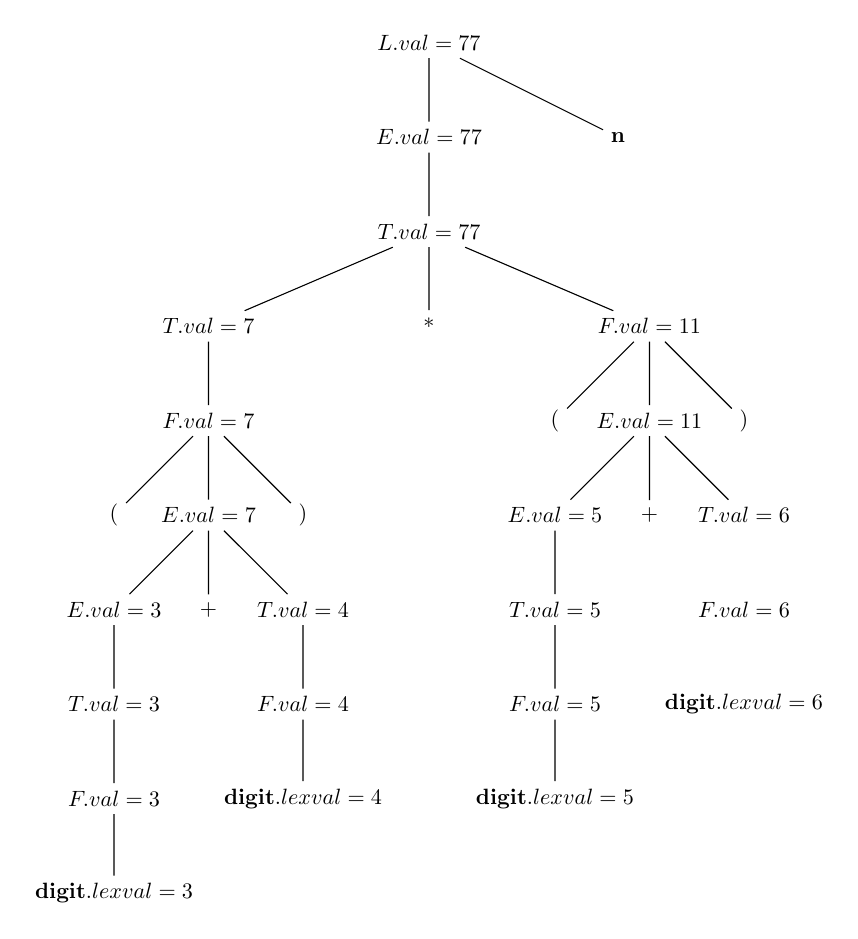
\begin{tikzpicture}[scale=0.8,every node/.style={scale=0.8}]
\node (v1) at (0,2.5) {$L.val=77$};
\node (v2) at (0,1) {$E.val=77$};
\node[font=\bfseries] (v3) at (3,1) {n};
\draw  (v1) edge (v2);
\draw  (v1) edge (v3);
\node (v4) at (0,-0.5) {$T.val=77$};
\draw  (v2) edge (v4);
\node (v6) at (0,-2) {*};
\node (v5) at (-3.5,-2) {$T.val=7$};
\node (v7) at (3.5,-2) {$F.val=11$};
\draw  (v4) edge (v5);
\draw  (v4) edge (v6);
\draw  (v4) edge (v7);
\node (v8) at (-3.5,-3.5) {$F.val=7$};
\draw  (v5) edge (v8);
\node (v10) at (-3.5,-5) {$E.val=7$};
\node (v9) at (-5,-5) {(};
\node (v11) at (-2,-5) {)};
\draw  (v8) edge (v9);
\draw  (v8) edge (v10);
\draw  (v8) edge (v11);
\node (v13) at (-3.5,-6.5) {+};
\node (v12) at (-5,-6.5) {$E.val=3$};
\node (v14) at (-2,-6.5) {$T.val=4$};
\draw  (v10) edge (v12);
\draw  (v10) edge (v13);
\draw  (v10) edge (v14);
\node (v15) at (-5,-8) {$T.val=3$};
\node (v16) at (-5,-9.5) {$F.val=3$};
\node (v17) at (-5,-11) {\textbf{digit}$.lexval=3$};
\draw  (v12) edge (v15);
\draw  (v15) edge (v16);
\draw  (v16) edge (v17);
\node (v18) at (-2,-8) {$F.val=4$};
\node (v19) at (-2,-9.5) {\textbf{digit}$.lexval=4$};
\draw  (v18) edge (v19);
\draw  (v14) edge (v18);
\node (v21) at (3.5,-3.5) {$E.val=11$};
\node (v20) at (2,-3.5) {(};
\node (v22) at (5,-3.5) {)};
\draw  (v7) edge (v20);
\draw  (v7) edge (v21);
\draw  (v7) edge (v22);
\node (v24) at (3.5,-5) {+};
\node (v23) at (2,-5) {$E.val=5$};
\node (v25) at (5,-5) {$T.val=6$};
\draw  (v21) edge (v23);
\draw  (v21) edge (v24);
\draw  (v21) edge (v25);
\node (v26) at (2,-6.5) {$T.val=5$};
\node (v27) at (2,-8) {$F.val=5$};
\node (v28) at (2,-9.5) {\textbf{digit}$.lexval=5$};
\draw  (v23) edge (v26);
\draw  (v26) edge (v27);
\draw  (v27) edge (v28);
\node at (5,-6.5) {$F.val=6$};
\node at (5,-8) {\textbf{digit}$.lexval=6$};
\end{tikzpicture}

    \end{figure}

    \item[2] 扩展图 5-4 中的 SDD,使它可以像图5-1所示的那样处理表达式
    \begin{table}[h]
        \centering
        \begin{tabular}{ll}
            \hline
            产生式 & 语义规则 \\
            \hline
            1) $T\rightarrow FT^\prime$ &
                $T^\prime .inh=F.val$\\
                & $T.val = T^\prime .syn$ \\
            2) $T^\prime \rightarrow *FT_1^\prime$ & $T_1^\prime .inh=T^\prime .inh\times F.val$\\
                & $T^\prime .syn=T_1^\prime .syn$\\
            3) $T^\prime \rightarrow \epsilon$ & $T^\prime .syn = T^\prime .inh$\\
            4) $F\rightarrow$\textbf{digit} & $F.val=$\textbf{digit}$.lexval$\\
            \hline
        \end{tabular} 
    \end{table}

    \sol 

    \begin{table}[H]
        \centering
        \begin{tabular}{ll}
            \hline
            产生式 & 语义规则 \\
            \hline
            1) $L\rightarrow E$\textbf{n} & $L.val=E.val$\\
            2) $E\rightarrow TE^\prime$ & $E^\prime .inh = T.val$ \\
            & $E.val=E^\prime .syn$\\
            3) $E^\prime \rightarrow +TE_1^\prime$ & $E_1^\prime .inh = E^\prime .inh + T.val$\\
            & $E^\prime .syn = E_1^\prime .syn$ \\
            4) $E^\prime \rightarrow \epsilon$ & $E^\prime .syn = E^\prime .inh$\\
            5) $T\rightarrow FT^\prime$ &
                $T^\prime .inh=F.val$\\
                & $T.val = T^\prime .syn$ \\
            6) $T^\prime \rightarrow *FT_1^\prime$ & $T_1^\prime .inh=T^\prime .inh\times F.val$\\
                & $T^\prime .syn=T_1^\prime .syn$\\
            7) $T^\prime \rightarrow \epsilon$ & $T^\prime .syn = T^\prime .inh$\\
            8) $F\rightarrow (E)$ & $F.val = E.val$\\
            9) $F\rightarrow$\textbf{digit} & $F.val=$\textbf{digit}$.lexval$\\
            \hline
        \end{tabular} 
    \end{table}

    \newpage
 
    \item[3] 使用你在上一题中得到的SDD,给出下列表达式对应的注释语法分析树:(3+4)*(5+6)\textbf{n}  
    
    \sol \begin{figure}[H]
        \centering
        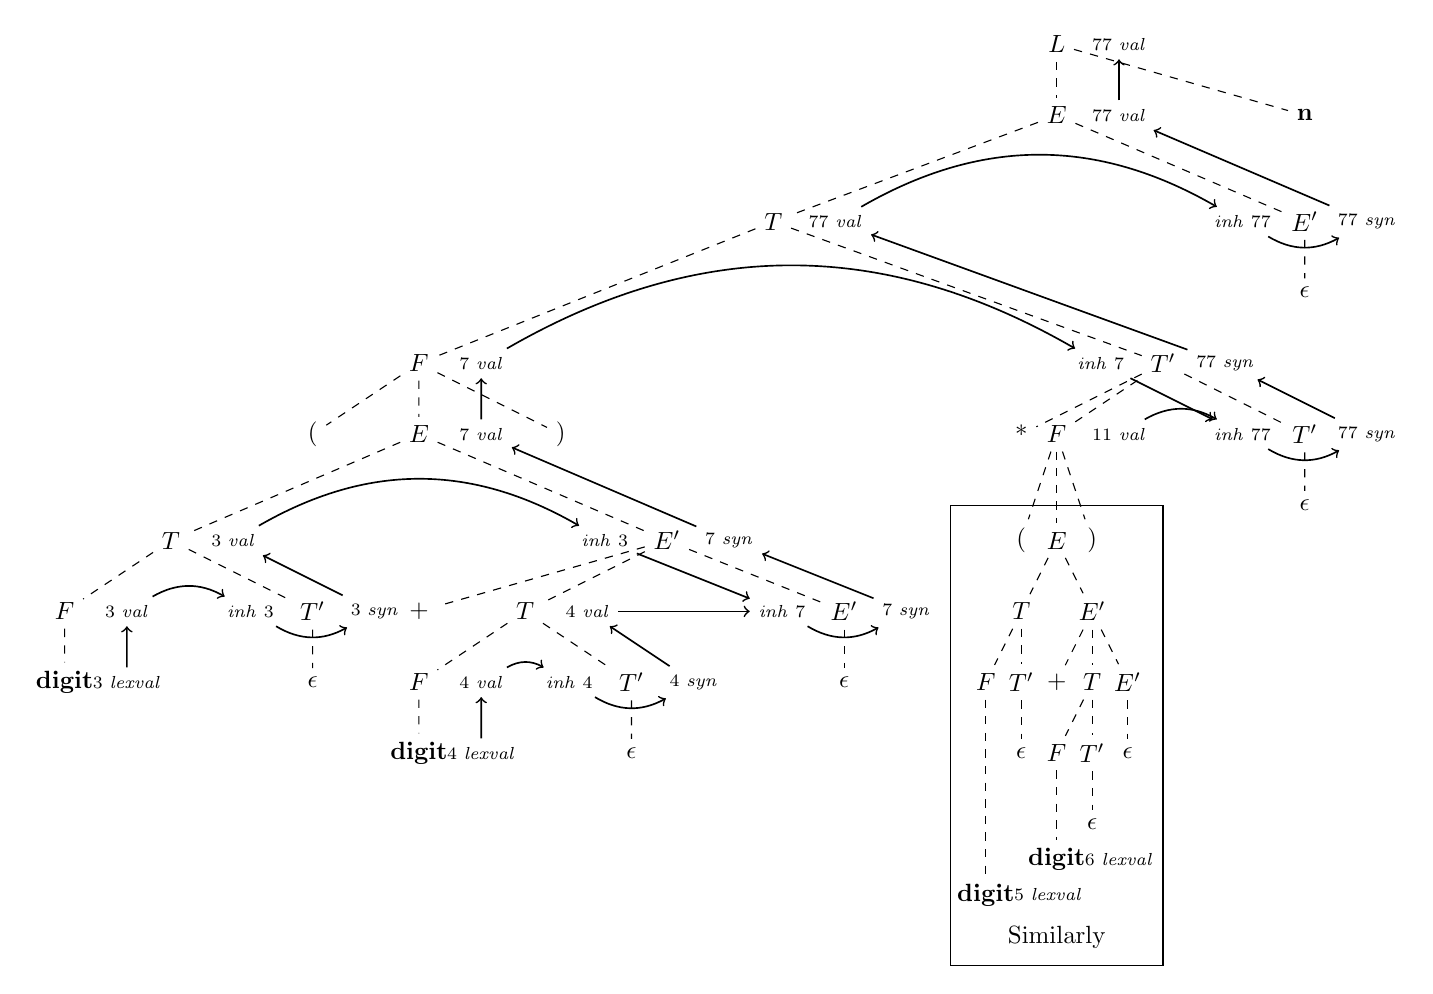
\begin{tikzpicture}[node distance=2.5em,scale=0.9,every node/.style={scale=0.9}]

\tikzstyle{calc}=[->,line width=0.6pt];
\tikzstyle{prop}=[font=\scriptsize];

\node (v1) at (1,5) {$L$};
\node (v1r) [prop,right of=v1] {77 \textit{val}};
\node (v2) at (1,4) {$E$};
\node (v2r) [prop,right of=v2] {77 \textit{val}};
\node[font=\bfseries] (v3) at (4.5,4) {n};

\draw [dashed] (v1) edge (v2);
\draw [dashed] (v1) edge (v3);
\node (v4) at (-3,2.5) {$T$};
\node (v4r) [prop,right of=v4] {77 \textit{val}};
\node (v5) at (4.5,2.5) {$E^\prime$};
\node (v5l) [prop,left of=v5] {\textit{inh} 77};
\node (v5r) [prop,right of=v5] {77 \textit{syn}};
\draw [dashed] (v2) edge (v4);
\draw [dashed] (v2) edge (v5);
\node (v6) at (4.5,1.5) {$\epsilon$};
\draw [dashed] (v5) edge (v6);
\node (v7) at (-8,0.5) {$F$};
\node (v7r) [prop,right of=v7] {7 \textit{val}};
\node (v8) at (2.5,0.5) {$T^\prime$};
\node (v8l) [prop,left of=v8] {\textit{inh} 7};
\node (v8r) [prop,right of=v8] {77 \textit{syn}};

\draw [dashed] (v4) edge (v7);
\draw [dashed] (v4) edge (v8);
\node (v9) at (0.5,-0.5) {*};
\node (v10) at (1,-0.5) {$F$};
\node (v10r) [prop,right of=v10] {11 \textit{val}};
\node (v11) at (4.5,-0.5) {$T^\prime$};
\node (v11l) [prop,left of=v11] {\textit{inh} 77};
\node (v11r) [prop,right of=v11] {77 \textit{syn}};
\draw [dashed] (v8) edge (v9);
\draw [dashed] (v10) edge (v8);
\draw [dashed] (v8) edge (v11);
\node (v12) at (-8,-0.5) {$E$};
\node (v12r) [prop,right of=v12] {7 \textit{val}};
\node (v13) at (-9.5,-0.5) {(};
\node (v14) at (-6,-0.5) {)};
\draw [dashed] (v7) edge (v12);
\draw [dashed] (v7) edge (v13);
\draw [dashed] (v7) edge (v14);
\node (v16) at (1,-2) {$E$};
\node (v15) at (0.5,-2) {(};
\node (v17) at (1.5,-2) {)};
\draw [dashed] (v10) edge (v15);
\draw [dashed] (v10) edge (v16);
\draw [dashed] (v10) edge (v17);
\node (v18) at (4.5,-1.5) {$\epsilon$};
\draw [dashed] (v11) edge (v18);
\node (v19) at (-11.5,-2) {$T$};
\node (v19r) [prop,right of=v19] {3 \textit{val}};
\node (v20) at (-4.5,-2) {$E^\prime$};
\node (v20l) [prop,left of=v20] {\textit{inh} 3};
\node (v20r) [prop,right of=v20] {7 \textit{syn}};
\node (v21) at (-8,-3) {+};
\node (v22) at (-6.5,-3) {$T$};
\node (v22r) [prop,right of=v22] {4 \textit{val}};
\node (v23) at (-2,-3) {$E^\prime$};
\node (v23l) [prop,left of=v23] {\textit{inh} 7};
\node (v23r) [prop,right of=v23] {7 \textit{syn}};
\draw [dashed] (v12) edge (v19);
\draw [dashed] (v12) edge (v20);
\draw [dashed] (v20) edge (v21);
\draw [dashed] (v20) edge (v22);
\draw [dashed] (v20) edge (v23);
\node (v24) at (-13,-3) {$F$};
\node (v24r) [prop,right of=v24] {3 \textit{val}};
\node (v25) at (-9.5,-3) {$T^\prime$};
\node (v25l) [prop,left of=v25] {\textit{inh} 3};
\node (v25r) [prop,right of=v25] {3 \textit{syn}};
\node (v26) at (-8,-4) {$F$};
\node (v26r) [prop,right of=v26] {4 \textit{val}};
\node (v27) at (-5,-4) {$T^\prime$};
\node (v27l) [prop,left of=v27] {\textit{inh} 4};
\node (v27r) [prop,right of=v27] {4 \textit{syn}};
\draw [dashed] (v19) edge (v24);
\draw [dashed] (v19) edge (v25);
\draw [dashed] (v22) edge (v26);
\draw [dashed] (v22) edge (v27);
\node [font=\bfseries] (v28) at (-13,-4) {digit};
\node (v28r) [prop,right of=v28] {3 \textit{lexval}};
\node [font=\bfseries] (v29) at (-8,-5) {digit};
\node (v29r) [prop,right of=v29] {4 \textit{lexval}};
\draw [dashed] (v24) edge (v28);
\draw [dashed] (v26) edge (v29);
\node (v30) at (-9.5,-4) {$\epsilon$};
\node (v31) at (-5,-5) {$\epsilon$};
\node (v32) at (-2,-4) {$\epsilon$};
\draw [dashed] (v25) edge (v30);
\draw [dashed] (v27) edge (v31);
\draw [dashed] (v23) edge (v32);

\draw[calc] (v28r) edge (v24r);
\draw[calc,bend left] (v24r) edge (v25l);
\draw[calc,bend right] (v25l) edge (v25r);
\draw[calc] (v25r) edge (v19r);
\draw[calc,bend left] (v19r) edge (v20l);
\draw[calc] (v29r) edge (v26r);
\draw[calc,bend left] (v26r) edge (v27l);
\draw[calc,bend right] (v27l) edge (v27r);
\draw[calc] (v27r) edge (v22r);
\draw[calc] (v22r) edge (v23l);
\draw[calc] (v20l) edge (v23l);
\draw[calc,bend right] (v23l) edge (v23r);
\draw[calc] (v23r) edge (v20r);
\draw[calc] (v20r) edge (v12r);
\draw[calc] (v12r) edge (v7r);
\draw[calc,bend left] (v7r) edge (v8l);
\draw[calc,bend left] (v10r) edge (v11l);
\draw[calc] (v8l) edge (v11l);
\draw[calc,bend right] (v11l) edge (v11r);
\draw[calc] (v11r) edge (v8r);
\draw[calc] (v8r) edge (v4r);
\draw[calc,bend left] (v4r) edge (v5l);
\draw[calc,bend right] (v5l) edge (v5r);
\draw[calc] (v5r) edge (v2r);
\draw[calc] (v2r) edge (v1r);

\node (v47) at (0.5,-3) {$T$};
\node (v48) at (1.5,-3) {$E^\prime$};
\node (v35) at (1,-4) {+};
\node (v36) at (1.5,-4) {$T$};
\node (v37) at (2,-4) {$E^\prime$};
%\draw [dashed] (v12) edge (v47);
%\draw [dashed] (v12) edge (v48);
\draw [dashed] (v48) edge (v35);
\draw [dashed] (v48) edge (v36);
\draw [dashed] (v48) edge (v37);
\node (v38) at (0,-4) {$F$};

\node (v39) at (0.5,-4) {$T^\prime$};
\node (v40) at (1,-5) {$F$};
\node (v41) at (1.5,-5) {$T^\prime$};
\draw [dashed] (v47) edge (v38);
\draw [dashed] (v47) edge (v39);
\draw [dashed] (v36) edge (v40);
\draw [dashed] (v36) edge (v41);
\node [font=\bfseries] (v42) at (0,-7) {digit};
\node (v42r) [prop,right of=v42] {5 \textit{lexval}};
\node [font=\bfseries] (v43) at (1,-6.5) {digit};
\node (v43r) [prop,right of=v43] {6 \textit{lexval}};
\draw [dashed] (v38) edge (v42);
\draw [dashed] (v40) edge (v43);
\node (v44) at (0.5,-5) {$\epsilon$};
\node (v45) at (1.5,-6) {$\epsilon$};
\node (v46) at (2,-5) {$\epsilon$};
\draw [dashed] (v39) edge (v44);
\draw [dashed] (v41) edge (v45);
\draw [dashed] (v37) edge (v46);
\draw [dashed] (v16) edge (v47);
\draw [dashed] (v16) edge (v48);
\draw  (-0.5,-1.5) rectangle (2.5,-8);
\node at (1,-7.6) {Similarly};
\end{tikzpicture}

    \end{figure}
\end{problems}

\end{document}
